\chapter{恒星的简并残骸}
上章讲到,大质量恒星超新星爆发后,会抛离周围大部分物质,中心留下简并核,根据核的质量不同会形成白矮星、中子星或黑洞等致密星。

\section{白矮星}
白矮星内部主要由电子简并压抵抗引力,其质量和太阳相当,但大小和地球差不多。白矮星内部没有核反应进行,表面温度5,000\,K到80,000\,K不等,同样我们根据白矮星的光谱可以将其分为五类:
\begin{itemize}
  \item DA,占总数的三分之二,有碰撞增宽的氢吸收线
  \item DB,占总数的$8\%$,只有氦吸收线
  \item DC,占总数的$14\%$,没有谱线的连续谱
  \item DQ,光谱中含碳线
  \item DZ,光谱中有金属线
\end{itemize}

\paragraph{白矮星冷却时标}
白矮星的电子由于简并,导致低能级占满,无法从更高能级下来,因此白矮星辐射的热量主要来自原子核的动能。因此假设白矮星质量为$M_\mathrm{wd}$,原子质量为$Am_H$,就可以得到原子数,因为每个原子核的内能是${2\over 3}kT$,就可以计算出总内能,配合白矮星的光度,可以得到
\begin{equation}
  \tau_\mathrm{cool}={U\over L_\mathrm{wd}}={3\over 2}{M_\mathrm{wd}k\over Am_H C T_c^{5/2}}
\end{equation}

代入典型值可以得到$\tau_\mathrm{cool}\approx 170$\;百万年,从式中还可知温度越低白矮星冷却的越慢,因此白矮星大部分时候以较低的温度和光度缓慢冷却。

\subsection{简并}
根据泡利不相容原理,不能有两个费米子具有相同的量子态,而能级的量子态总数是有限的。因此当物质的密度很大时,会产生简并压,以防止更多的粒子被压至相同的轨道。那么简并压是否有上限?

由于费米子除了遵循泡利不相容原理,还要符合海森堡不确定性原理,因此当电子被压得相互之间很靠近时,其位置不确定性会减小,动量的不确定性会增加,速度也因此增加,而速度的最大不能超过光速,这就是简并压的上线。

1931年,印度物理学家钱德拉塞卡由此计算了电子简并压的上限,并提出了白矮星的质量上限——\textbf{钱德拉塞卡极限}$M_\mathrm{Ch}=1.44\,M_\odot$。

\section{中子星}
那么当白矮星的质量超过钱德拉塞卡极限之后会怎么样?电子会被压缩进原子核,与质子合并形成中子,中子星就由此诞生了。

一颗质量与太阳相当的中子星,直径大约只有10\,km。中子星内部由中子简并压抵抗引力,由于中子具有比电子更大的质量,因此它的简并压上线比电子大得多。同时由于体积的压缩,为了满足磁通量守恒,中子星的磁场非常强$B\sim10^{12}\,$G。

\section{脉冲星}
脉冲星是一类特殊的天体,观测上表现为周期性的脉冲信号,并且周期很短,最低达到毫秒量级,最高在秒量级。

目前大家公认为是脉冲星本质是中子星,如图\ref{fig:pulsar},中子星的磁场也是偶极磁场,被磁场捕获的带电粒子在沿两极被抛出,这就是脉冲的来源。而在白矮星塌缩至中子星的过程中,也要满足角动量守恒,因此中子星的自转周期非常短,这也解释了脉冲星短周期的原因。

\begin{figure}[hbt]
  \centering
  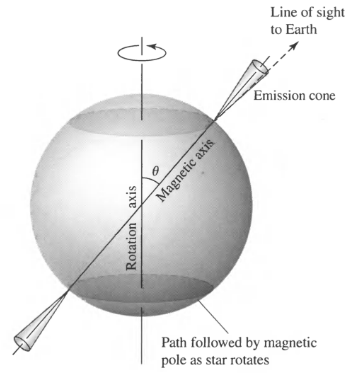
\includegraphics[width=8cm]{chapters/16/pulsar}
  \caption{基本的脉冲星模型}
  \label{fig:pulsar}
\end{figure}

由于脉冲星周围的强磁场,当捕获带电粒子之后,带电粒子绕旋磁场线运动,会产生辐射。如果捕获的是相对论性(速度接近光速)带电粒子,会产生\textbf{同步辐射};如果磁场很强,或带电粒子的入射角很小,导致回旋半径很小,那么带电粒子就好像是沿着磁场线运动一样,这时产生的是\textbf{曲率辐射}。

脉冲星中还有一类特殊的群体——\textbf{软伽马射线复现源},这类被认为是由具有更强磁场的中子星——\textbf{磁星}所产生的

\paragraph{光速圆柱面(光柱面)}
带电粒子被中子星磁场捕获后,会随着磁场与中子星同步转动,但在距离中子星自转轴$R_c=c/\omega=cP/2\pi$处,如图\ref{fig:lightcylinder},同步速度达到光速,带电粒子无法继续没束缚,就会被甩出去,并产生同步辐射或曲率辐射。

\begin{figure}[hbt]
  \centering
  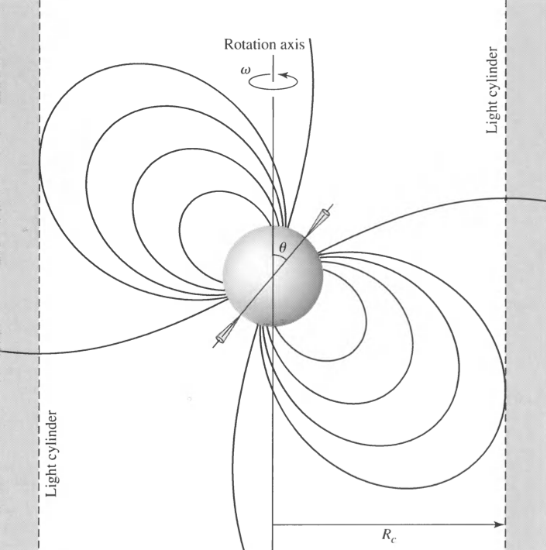
\includegraphics[width=10cm]{chapters/16/lightcylinder}
  \caption{中子星周围的\textbf{光柱面}。}
  \label{fig:lightcylinder}
\end{figure}
